\chapter{Methodology}

\begin{figure}
   \centering
   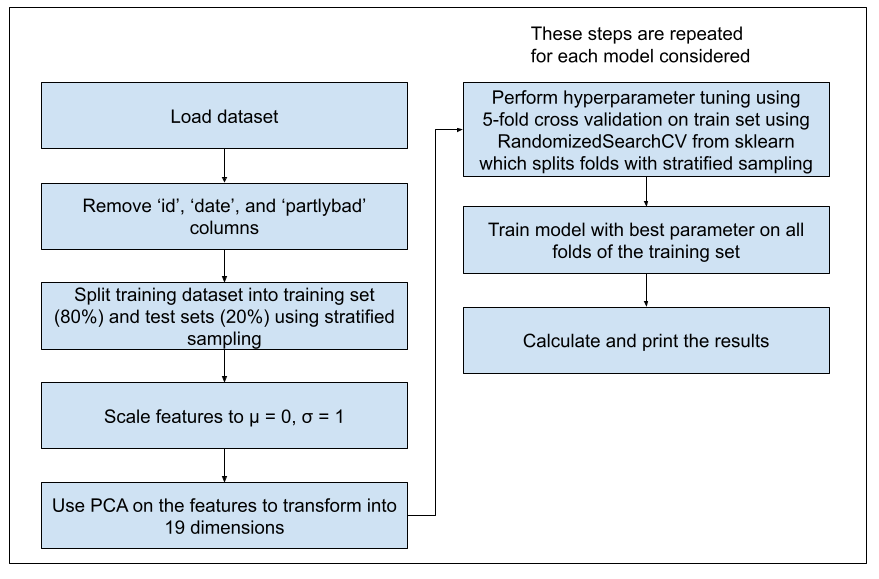
\includegraphics[width=0.9\textwidth]{images/pipeline.png}
   \caption{Machine learning pipeline}
   \label{fig:pipeline}
\end{figure}

Figure \ref{fig:pipeline} illustrates the machine learning pipeline which consists of nine steps. First, datasets \textit{npf\_train.csv} and \textit{npf\_test.csv} are downloaded. We remove the unnecessary columns, including 'id', 'date', and 'partlybad'. 'id' was removed because this provides no information and would lead to model overfitting on the field since it is unique for each example. 'partlybad', opposite of 'id', consists of all examples having the same value. 'date' was removed because this is not present in the test dataset.

Next, we split the npf\_train.csv dataset into two stratified parts identically as discussed previously when performing exploratory data analysis, that is, 80\% for training and 20\% for test sets.

After that, we standardize the features to mean zero and unit variance. This scaler is fit on the train set and then applied to the test set. We reduce the dimension of our data by using principal component analysis (PCA). Similarly to scaling, we fit PCA on the training subset to the 19 components as apply that to the test subset. At this stage, we have four datasets: training and test sets with original data, and training and test sets with PCA. We keep all four to see how dimensionality reduction affects our models. The next step is to train our models.

For each model, we perform 5-fold cross-validation hyperparameter tuning using \textit{RandomizedSearchCV} from sklearn. This automatically splits the folds with stratified sampling. After that, the model with the best hyperparameters is trained on the train set and then evaluated on the test set. The results of each model will be discussed in the next section. Before that, we give a brief overview of the models we used.

\section{Models}

This section describes each of the models we used. The first type of models we used is the generative Gaussian Naive Bayes. The goal of generative models is to describe how data is created. The model relies on Bayes theorem and uses parameters that maximizes the joint probability between the features and the target variable P(X, Y) to train the model.

The second type of models used are discriminative. The goal of discriminative models is to predict the labels of the data. The model learns boundaries between classes in a dataset and trains a model using parameters that maximize the conditional probability of the target variable given the features P(x \textbar Y). Below, we list the discriminative models used. It can be noticed that some of the models contain "with class balanced weights". This means that the weights for each example is set inversely proportionate to their relative frequencies. This can be done in \textit{scikit-learn} by setting the \textit{class\_weight} parameter to 'balanced'.

\begin{itemize}
	\item Logistic Regression - Used to understand the relationship between variables and uses previous data to estimate an event's probability. Assumes a linear relationship between each feature and the target variable
	\item Logistic Regression with class balanced weights
	\item Support Vector Machine (SVM) - An algorithm that divides n-dimensional space into classes by establishing a decision boundary. A hyperplane is the best decision boundary, and it is constructed by choosing the extreme points that are called support vectors
  
  \item Support Vector Machine with class balanced weights
  
  \item Decision Tree - Has the objective to learn basic decision rules from data features to create a model that predicts the target variable's value. It can handle both numerical and categorical data
  
  \item Decision Tree with class balanced weights
  
  \item Random Forest (RF)- Employs averaging to increase predicted accuracy and control over-fitting by fitting decision tree classifiers on sub-samples of the dataset.
  
  \item Random Forest with class balanced weights
  
  \item Multi-Layer Perceptron (MLP)- Used neural networks to perform the classification task.
  
\end{itemize}
